\chapter{The LHC and the CMS Detector}
\label{chap:cmsoverview}

Probing the \SM for signs of new physics would not be possible without the immensely complex electronics and machinery that makes the TeV energy scale accessible for the first time. This chapter will cover \CERN 's  Large Hadron Collider (\LHC) and the CMS detector, being the experiment the author is a member of. Section \ref{sec:cmsdetector} serves to introduce an overview of the different components of  the CMS detector, with more detail spent on those that are relevant in the search for Supersymmetric particles. Section \ref{sec:cmsobjects} will focus on event and object reconstruction again with more emphasis on jet level quantities which are most relevant to the author's analysis research. Finally Section \ref{sec:triggersystem} will cover work performed by the author, as service to the CMS Collaboration, in measuring the performance of the GCT component of the L1 trigger during the 2012-2013 run period.  


\section{The LHC}
\label{sec:thelhc} 

The \LHC is a storage ring, accelerator, and collider of circulating beams of protons or ions. Housed in the tunnel dug for the Large Electron-Positron collider (LEP), it is approximately 27 km in circumference, 100 m underground, and straddles the border between France and Switzerland outside of Geneva. It is currently the only collider in operation that is able to study physics at the TeV scale.  A double-ring circular synchrotron, it was
designed to collide both proton-proton (pp) and heavy ion (PbPb) with a centre of mass energy $\sqrt{s} = $ 14 \TeV at a final design luminosity of $10^{34}$cm$^{-2}$s$^{-1}$. \\

These counter-circulating beams of protons/Pb ions are merged in four sections around the ring to enable collisions of the beams, with each interaction point being home to one of the four major experiments; ALICE \cite{alicetdr} , ATLAS \cite{atlastdr}, CMS \cite{cmstdr} and LHCb \cite{lhcbtdr} which record the resultant collisions. The layout of the \LHC ring is shown in Figure \ref{fig:lhc-ring}. The remaining four sections contain acceleration,collimation and beam dump systems. In the eight arc sections, the beams are steered by magnetic fields of up to 8 \T provided by super conduction dipole magnets, which are maintained at temperatures of 2 \K using superfluid helium. Additional magnets for focusing and corrections are also present in straight sections within the arcs and near the interaction regions where the detectors are situated. \\


\begin{figure}[!h]

\centering
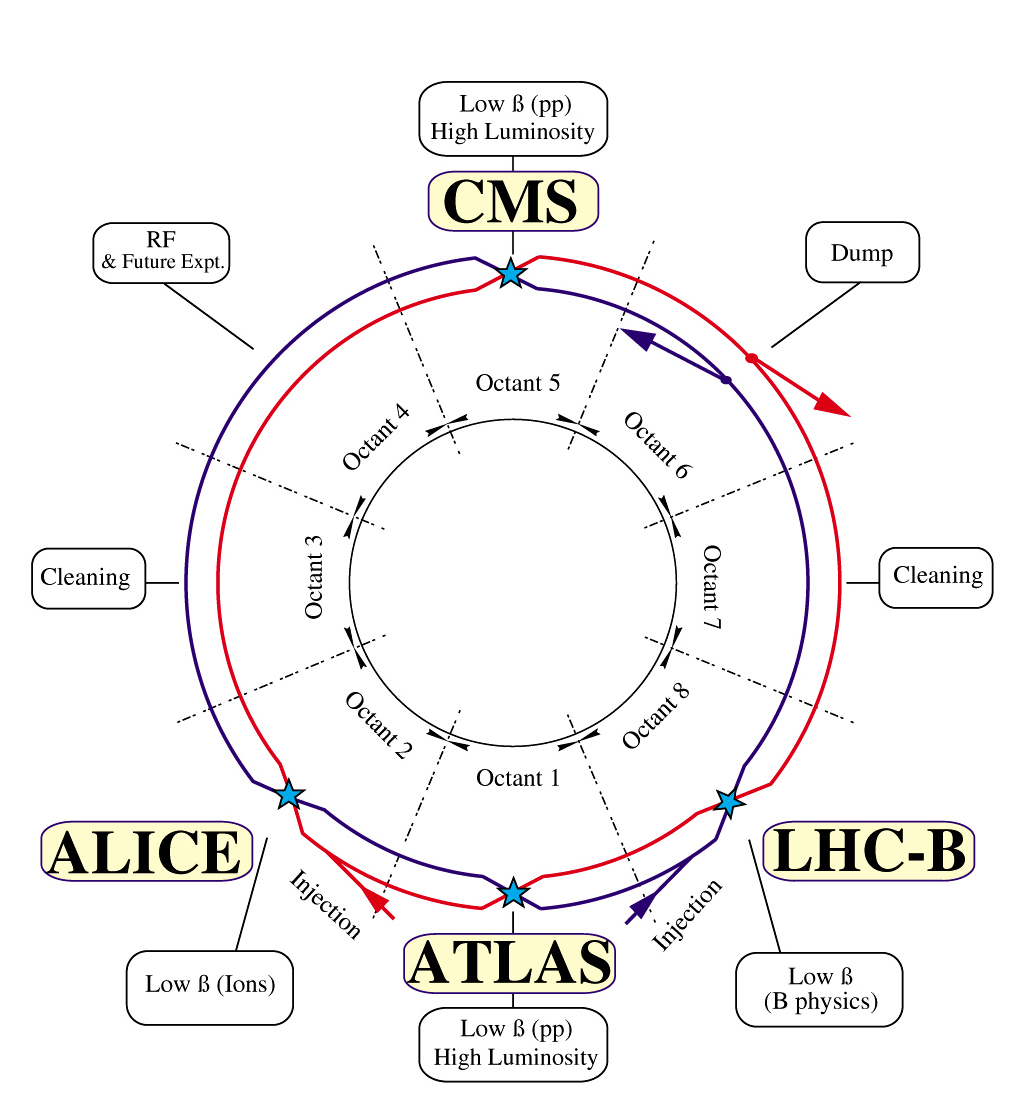
\includegraphics[width=0.65\textwidth]{plots/lhc-ring-photo.png}
\caption[A top down layout of the \LHC.]{A top down layout of the \LHC. \cite{Jean-Luc:841573}}  
\label{fig:lhc-ring}
\end{figure}


Proton beams are formed inside the Proton Synchrotron (PS) from bunches of protons 50 \ns apart with an energy of 26 \GeV. The protons are then accelerated in the Super Proton Synchrotron(SPS) to 450 \GeV  before being injected into the \LHC. These \LHC proton beams consists of many "bunches" i.e. approximately $1.1 \times 10^{11}$  protons localized into less than 1 \ns in the direction of motion. Before collision the beams are ramped to 4 \TeV (2012) per beam in a process involving increasing the current passing through the dipole magnets. Once the desired \com energy is reached then the beams are allowed to collide at the interaction points. The luminosity falls regularly as the run progresses as protons are lost in collisions, and eventually the beam is dumped before repeating the process again. \\

In the early phase of prolonged operation after the initial shutdown the machine operated in 2010-2011 at 3.5 \TeV per beam, \com $=$ 7 \TeV, delivering 6.13 \fb of data \cite{LHClumo}. During the 2012-2013 run period, data was collected at an increased \com $=$ 8 \TeV improving the sensitivity of searches for new physics. Over the whole run period 23.3 \fb of data was delivered of which 21.8 \fb was recorded by the \CMS detector \cite{LHClumo}. A total of 12 \fb of 8 \TeV certified data was collected by October 2012, and it is this data which forms the basis of the results discussed within this thesis.

\begin{figure}[!h]

\centering
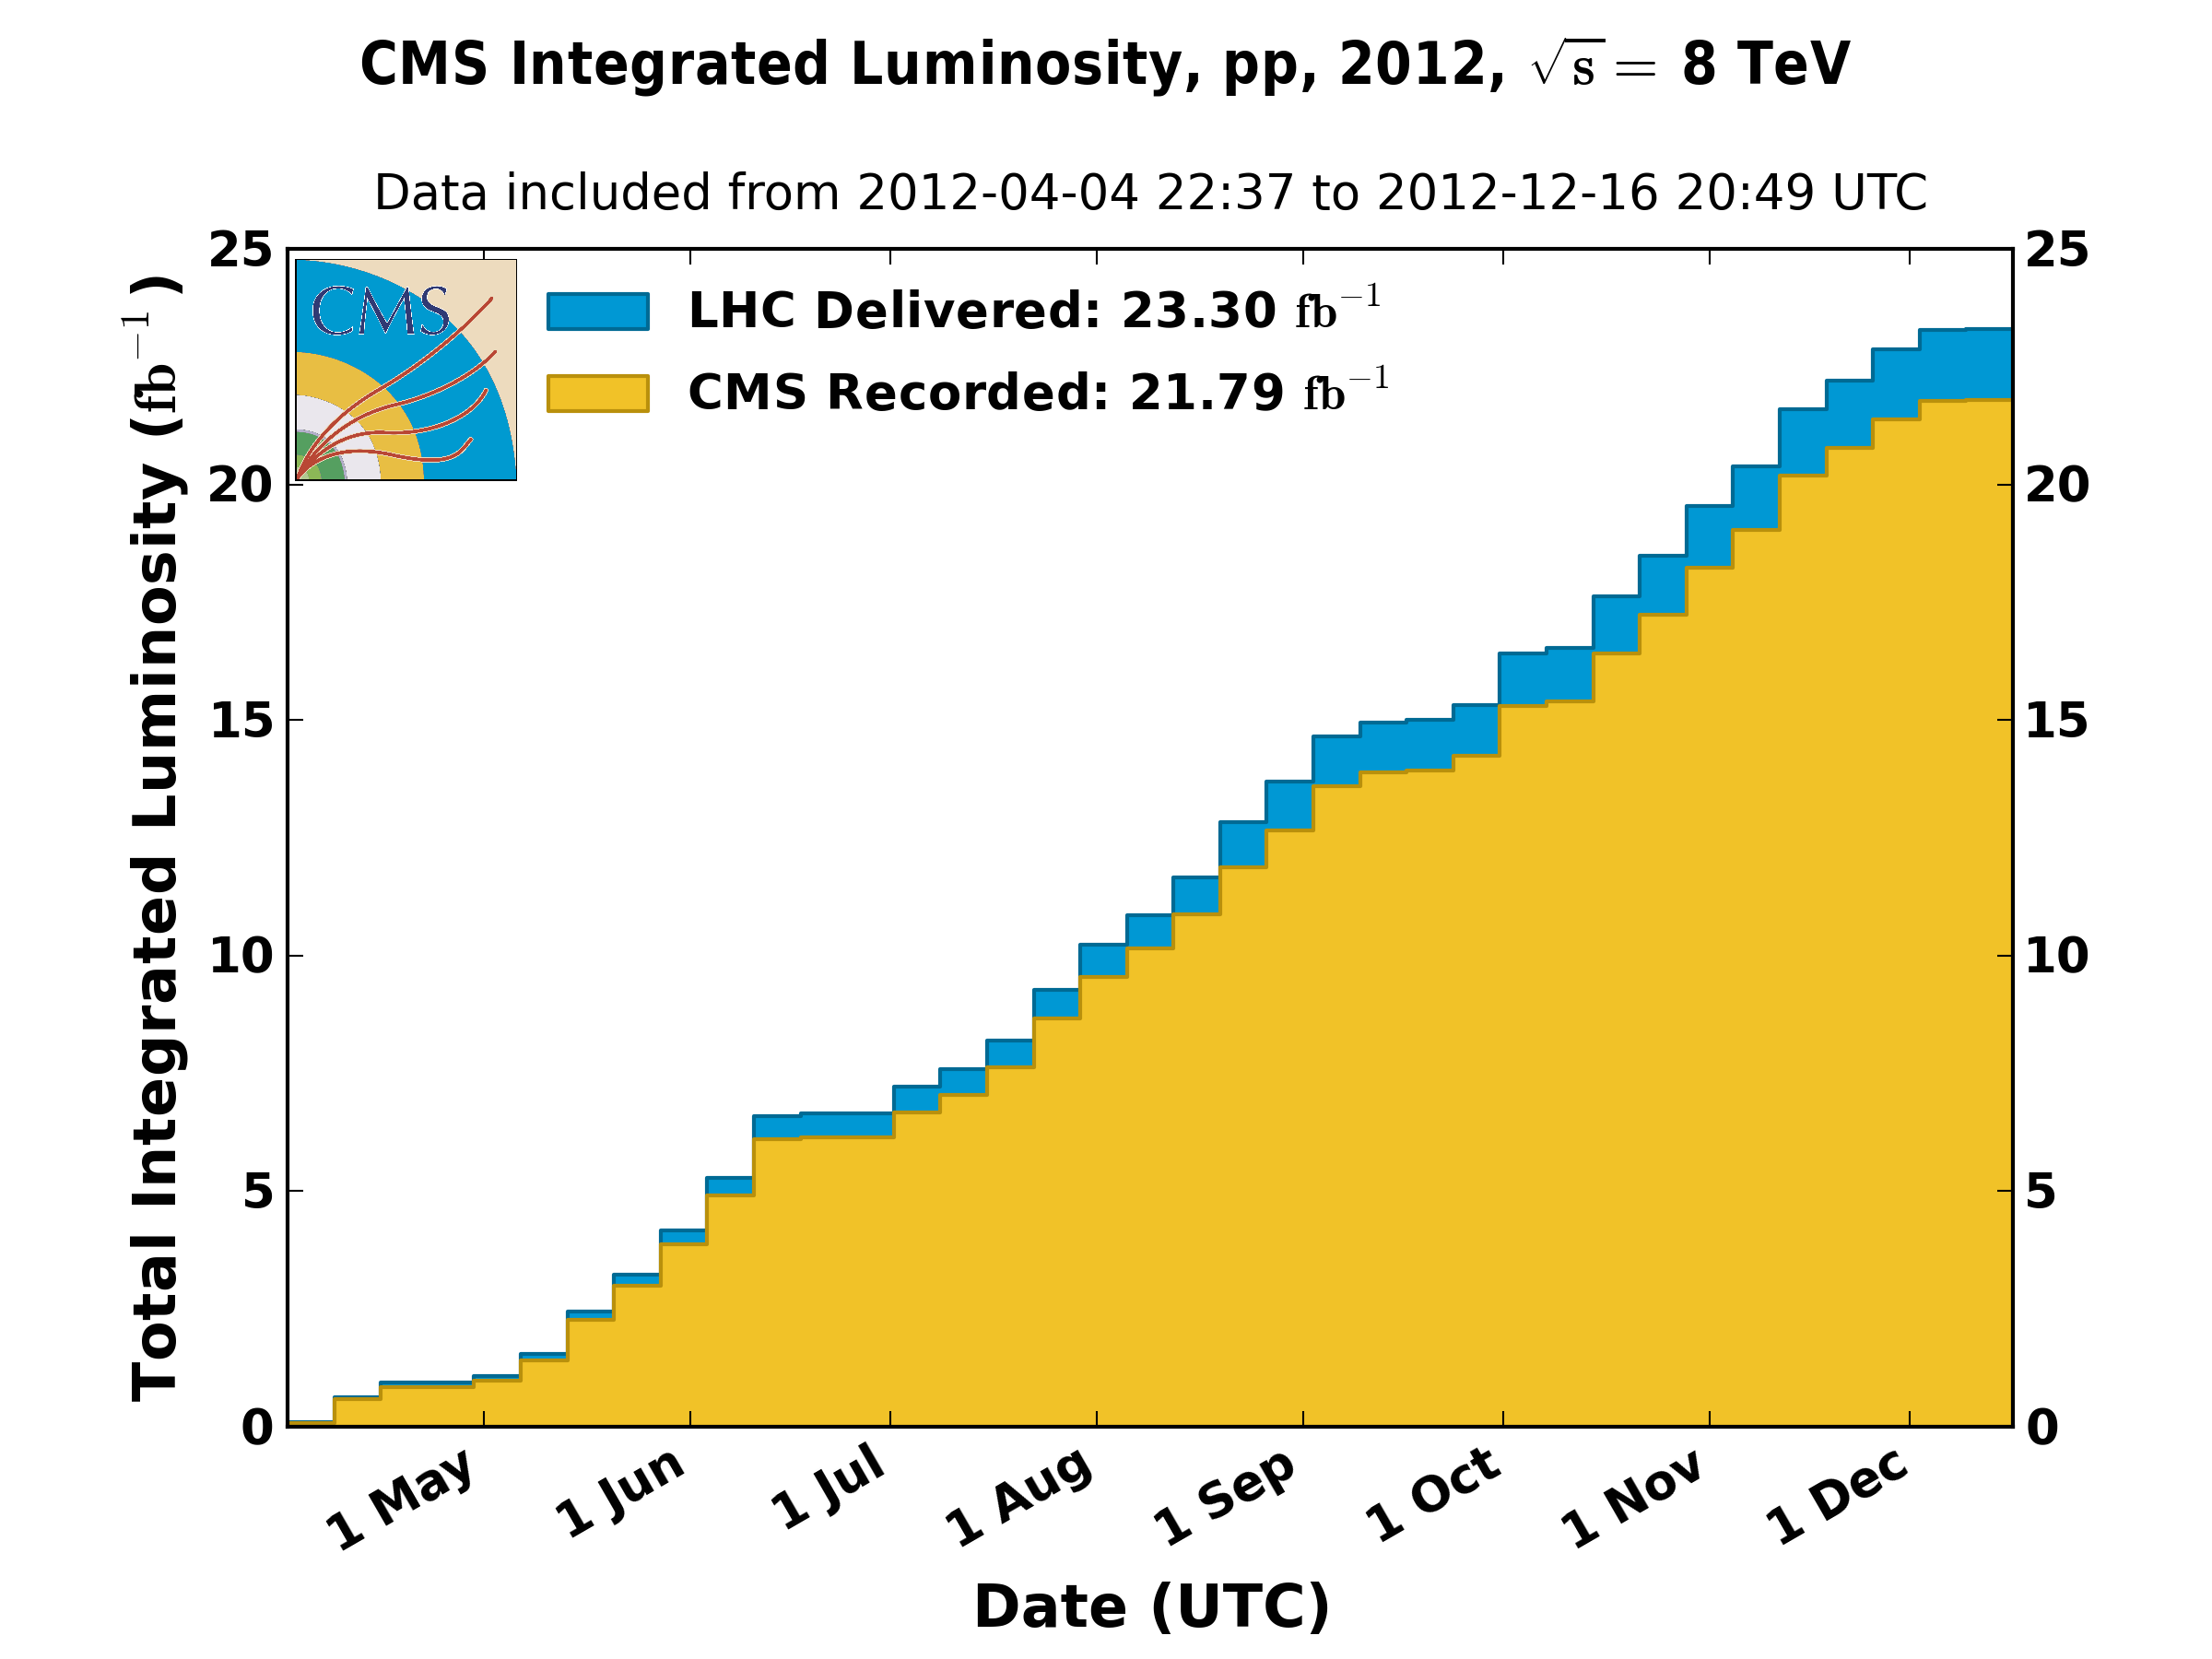
\includegraphics[width=0.65\textwidth]{plots/lhc-lumo-8tev.png}
\caption[The total integrated luminosity delivered to and collected by \CMS during the 2012 8 \TeV \pp runs]{The total integrated luminosity delivered to and collected by \CMS during the 2012 8 \TeV \pp runs.}  
\label{fig:lhc-ring}
\end{figure}


\section{The CMS detector}
\label{sec:cmsdetector}

The Compact Muon Solenoid (\CMS) detector is one of two general purpose detectors at the \LHC designed to search for new physics. The detector is designed to provide efficient identification and measurement of many physics objects including photons, electrons, muons, taus, and hadronic showers over wide ranges of transverse momentum and direction. Its nearly 4$\pi$ coverage in solid angle allows for accurate measurement of global transverse momentum imbalance. These design factors give \CMS the ability to search for direct production of \SUSY particles at the \TeV scale, making the search for Supersymmetric particles one of the highest priorities among the wide range of physics programmes at \CMS. \\

\CMS uses a right-handed Cartesian coordinate system with the origin at the interaction point and the z-axis pointing along the beam axis, the x-axis points radially inwards to the centre of the collider ring, with the y-axis points vertically upward. The azimuthal angle, $\phi$ ranging between [$-\pi$,$\pi$] is defined in the x-y plane starting from the x-axis. The polar angle $\theta$ is measured from the z axis. The common convention in particle physics is to express an out going particle in terms of $\phi$ and its pseudorapidity defined as

\begin{equation}
\eta = -\log\tan\left(\frac{\theta}{2}\right).
\end{equation}

The variable $\Delta R = \sqrt{\Delta\phi^{2} + \Delta\eta^{2} } $ is commonly used to define angular distance between objects within the detector and additionally energy and momentum is typically measured in the transverse plane perpendicular to the beam line. These values are calculated from the x and y components of the object and are denoted as $\et = E\sin\theta$ and $\pt = \sqrt{p^{2}_{x}+p^{2}_{y}}$. 

\subsection{Detector Subsytems}
\label{subsec:detectorsubsystems}

As the range of particles produced in \pp collisions interact in different ways with matter, \CMS is divided into subdetector systems, which perform complementary roles to identify the identity, mass and momentum of the different physics objects present in each event. These detector sub-systems contained inside \CMS are wrapped in layers around a central 13 m long 4 \T super conducting solenoid as shown in Fig \ref{fig:cms-detector}. With the endcaps closed , \CMS is a cylinder of length 22 m, diameter 15 m, and mass 12.5 kilotons. A more detailed complete description of the detector can be found elsewhere \cite{cmstdr}. \\

\begin{figure}[!h]

\centering
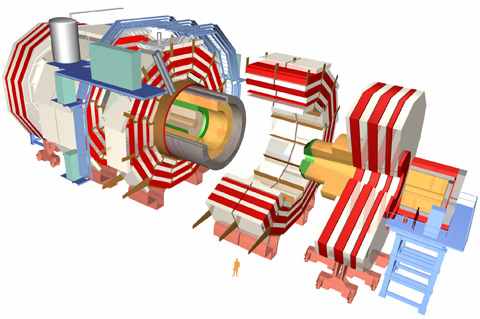
\includegraphics[width=0.65\textwidth]{plots/cms-detector.png}
\caption[A pictorial depiction of the \CMS detector.]{A pictorial depiction of the \CMS detector with the main detector subsystems labelled.   \cite{cms-public-detector}}  
\label{fig:cms-detector}
\end{figure}

\subsection{Tracker}
\label{subsec:tracker}

 The inner-most subdetector of the barrel is the multi-layer silicon tracker, formed of a pixel detector component encased by layers of silicon strip detectors. The pixel detector consists of three layers of silicon pixel sensors providing measurements of the momentum, position coordinates of the charged particles as they pass, and the location of primary and secondary vertices between 4cm and 10cm transverse to the beam. Outside the pixel detector, ten cylindrical layers of silicon strip detectors extend the tracking system out to a radius of 1.20m from the beam line. The tracking system provides efficient and precise determination of the charges, momenta, and impact parameters of charged particles with the geometry of the tracker extending to cover a rapidity range up to $\lvert\eta\rvert \textless$ 2.5.  \\
 
 The tracking system also plays a crucial part in the identification of jets originating from b-quarks through measurement of displaced secondary vertices, which is covered in more detail in Section \ref{subsec:cmsobjects-btagging}. The identification of b-jets is important in many searches for natural \SUSY models and forms an important part of the inclusive search strategy described within Section \ref{subsec:searchstrategy}.
 
\subsection{Electromagnetic Calorimeter}
\label{subsec:ecal}

 Immediately outside of the tracker, but still within the magnet core, sits the Electromagnetic Calorimeter (\ECAL). Covering a pseudorapididity up to $\lvert\eta\rvert < 3$ and compromising of over 75,000 PbWO$_{4}$ (lead tungstate) crystals that scintillate as particles deposit energy, the \ECAL provides high resolution measurements of the electromagnetic showers from photons, electrons in the detector. \\ 
 
 Lead tungstate is used because of its short radiation length ($X_{0} \sim 0.9$cm) and small Molier\'{e} radius ($\sim 2.1$cm) leading to high granularity and resolution. It's fast scintillation time ($\sim 25$ns) reduces the effects of pileup due to energy from previous collisions still being read out, and its radiation hardness gives it longevity. The crystals are arranged in modules which surround the beam line in a non-projective geometry,  angled at 3$^{\circ}$ with respect to the interaction point to minimise the risk of particles escaping down the cracks between the crystals.\\
 
 The  \ECAL is primarily composed of two sections, the Electromagnetic Calorimeter Barrel (\EB) which extends in pseudo-rapidity to $\lvert\eta\rvert < 1.479$ with a crystal front cross section of 22 $\times$ 22 mm$^{2}$ and a length of 230 mm corresponding to 25.8 radiation lengths, and the Electronmagnetic Calorimeter Endcaps (\EE) covering a rapidity range of $1.479 < \lvert\eta\rvert < 3.0 $, which consists of two identical detectors
on either side of the EB.  A lead-silicon sampling 'pre-shower' detector (\ES) is placed before the endcaps to aid in the identification of neutral pions. Their arrangement are shown in Figure \ref{fig:cms-ecal}. \\

 
 \begin{figure}[!h]

\centering
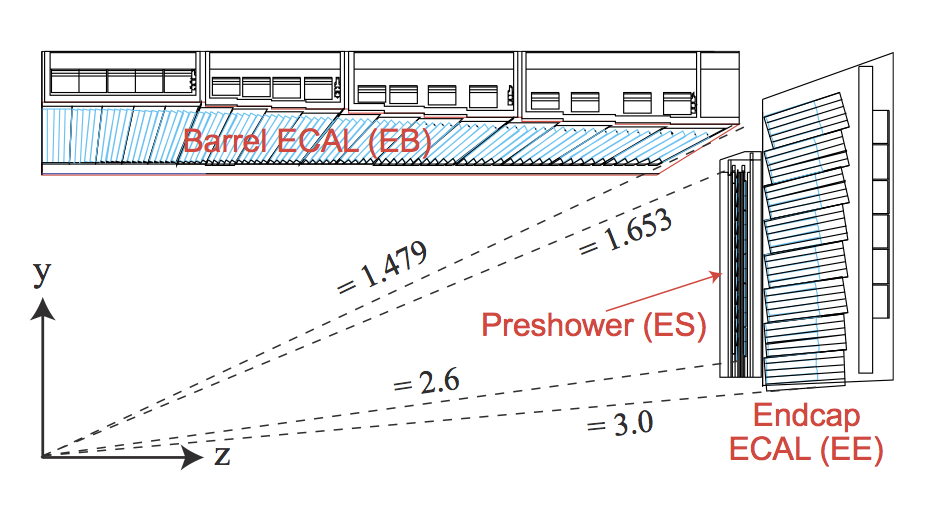
\includegraphics[width=0.85\textwidth]{plots/cms-ecal.png}
\caption[Illustration of the \CMS \ECAL showing the arrangement of the lead tungstate crystals in the \EB and \EE. The \ES is also shown and is located infront of the \EE.]{Illustration of the \CMS \ECAL showing the arrangement of the lead tungstate crystals in the \EB and \EE. The \ES is also shown and is located infront of the \EE \cite{CMS_ECAL_TDR}.}  
\label{fig:cms-ecal}
\end{figure}


Scintillation photons from the lead tungstate crystals are instrumented with avalanche photo-diodes (\APD) and vacuum photo-triodes (\VPT) located in the \EB and \EE respectively, converting the scintillating light into an electric signal which is consequently used to determine the amount of energy deposited within the crystal . These instruments are chosen for their resistance under operation to the strong magnetic field of \CMS. The scintillation of the \ECAL crystals as well as the response of the \APD s varies as a function of temperature and so cooling systems continually maintain an overall constant \ECAL temperature $\pm 0.05 ^{\circ}C$.
 

\subsection{Hadronic Calorimeter}
\label{subsec:hcal} 

Beyond the \ECAL lies the Hadronic Calorimeter (\HCAL), which is responsible for the accurate measurement of hadronic showers, crucial for analyses involving jets or missing energy signatures. The \HCAL is a sampling calorimeter which consists of alternating layers of brass absorber and plastic scintillator, except in the hadron forward ($3.0 < \lvert\eta\rvert < 5.0 $) region in which steel absorbers and quartz fibre scintillators are used because of their increased radiation tolerance. Hadron showers are initiated in the absorber layers inducing scintillation in the plastic scintillator tiles.  These scintillation photons are converted by wavelength shifting fibres for read-out by hybrid photodiodes. \\

The \HCAL's size is constrained to a compact size by the presence of the solenoid, requiring the placement of an additional outer calorimeter on the outside of the solenoid to increase the sampling depth of the \HCAL. A schematic of the \HCAL can be seen in Figure \ref{fig:cms-hcal}.\\
 
 \begin{figure}[!h]

\centering
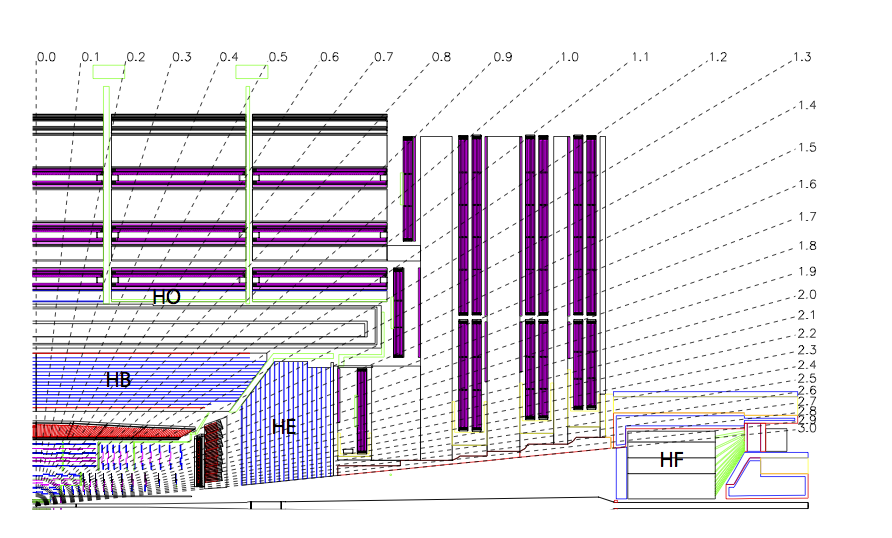
\includegraphics[width=0.85\textwidth]{plots/cms-hcal.png}
\caption[Schematic of the hadron calorimeters in the r-z plane, showing the locations of the HCAL components and the HF]{ Schematic of the hadron calorimeters in the r-z plane, showing the locations of the HCAL components and the HF. \cite{cmstdr}.}  
\label{fig:cms-hcal}
\end{figure}
 
The HCAL covers the range $\lvert\eta\rvert < 5$ and consists of four subdetectors: the Hadron Barrel (\HB)  $\lvert\eta\rvert < 1.3$, the Hadron Outer (\HO), the Hadron Endcap (\HE) $1.3 < \lvert\eta\rvert < 3.0 $ and the Hadron Forward (\HF).  The \HB is contained between the outer edge of the \ECAL and the inner edge of the solenoid, formed of 36 azimuthal wedges it is split between two half-barrel segments. The relatively short number of interaction lengths ($\lambda_{l}$, the distance a hadron will travel through the absorber material before it has lost $\frac{1}{e}$ of its energy) within the \HB, the lowest being $\lambda_{l}$ = 5.82 for $\lvert\eta\rvert = 0$, facilitates the need for the 'tail catching' \HO to increase the sampling depth in the central barrel rapidity region $\lvert\eta\rvert < 1.3$ to 11 interaction lengths . Significant fractions of the hadrons energy will be deposited in the \ECAL as it passed through the detector. Therefore measurements of hadron energies in the central regions $\lvert\eta\rvert < 3.0$ use both the \ECAL and \HCAL to reconstruct the true energy from showering hadrons. 

\subsection{Muon Systems}
\label{subsec:muonsystems} 
 
Muons being too massive to radiate away energy via Bremsstrahlung, interact little in the calorimeters and mostly pass through the detector until they reach the system of muon detectors which forms the outer most part of the \CMS detector.  

Outside of the superconducting solenoid are four muon detection layers interleaved with the iron return yokes which measure the muons energy via ionisation of gas within detector elements. Three types of gaseous chamber are used. The drift tube (\DT), cathode strip chamber (\CSC), and resistive plate chamber (\RPC) systems provide efficient detection of muons with pseudo-rapidity $\lvert\eta\rvert < 2.4 $. The best reconstruction performance is obtained when the muon chamber is combined with the inner tracking information to determine muon trajectories and their momenta \cite{CMS_MUON_TDR}.  \\ 


\section{Event Reconstruction and Object Definition}
\label{sec:cmsobjects}

The goal of event reconstruction is to take the raw information recorded by the detector and to compute from it higher-level quantities which can be used at an analysis level. These typically correspond to an individual particle's energy and momenta, or groups of particles which shower in a narrow cone and the overall global energy and momentum balance of the event. The reconstruction of these objects are described in great detail in \cite{CMS_TDR_PHYS_vol1}, however covered below are brief descriptions of those which are most relevant to the analysis detailed in Section \ref{chap:SUSYsearches}.

\subsection{Jets}
\label{subsec:cmsobjects-jets}

Quarks and gluons are produced copiously at the LHC in the hard scattering of partons. As these quarks and gluons fragment, they hadronise to form jets of strongly interactive particles and their decay products.  Jets are reconstructed from energy deposits in the detector using the anti-kt algorithm \cite{antiktalgo} with size parameter $\Delta R = 0.5$. The anti-kt jet algorithm clusters, 

Calorimeter jets are reconstructed using energy deposits in the electromagnetic (\ECAL) and hadronic (\HCAL) calorimeter cells, combined into calorimeter towers  \cite{Janssen:1322145}.


\subsection{B-tagging}
\label{subsec:cmsobjects-btagging}

The decays of b quarks are suppressed by small \CKM matrix elements. As a result, the lifetimes of b-flavoured hadrons, produced in the fragmentation of b quarks, are relatively long; $\mathcal{O}$ 1ps. Testing

\section{Triggering System}
\label{sec:triggersystem}

\subsection{L1 Trigger}
\label{subsec:l1trigger}

L1 Work
